
\chapter{Pneumatic instrumentation} 

While electricity is commonly used as a medium for transferring energy across long distances, it is also used in instrumentation to transfer \textit{information}.  A simple 4-20 mA current ``loop'' uses direct current to represent a process measurement in percentage of span, such as in this example: \index{4 to 20 mA}

$$\includegraphics{pneumatics00.eps}$$

The transmitter senses an applied fluid pressure from the process being measured, regulates electric current in the series circuit according to its calibration (4 mA = no pressure ; 20 mA = full pressure), and the indicator (ammeter) registers this measurement on a scale calibrated to read in pressure units.  If the calibrated range of the pressure transmitter is 0 to 250 PSI, then the indicator's scale will be labeled to read from 0 to 250 PSI as well.  No human operator reading that scale need worry about how the measurement gets from the process to the indicator -- the 4-20 mA signal medium is transparent to the end-user as it should be.

\vskip 10pt

\filbreak

Air pressure may be used as an alternative signaling medium to electricity.  Imagine a pressure transmitter designed to output a \textit{variable air pressure} according to its calibration rather than a \textit{variable electric current}.  Such a transmitter would have to be supplied with a source of constant-pressure compressed air instead of an electric voltage, and the resulting output signal would be conveyed to the indicator via tubing instead of wires:

$$\includegraphics{pneumatics01.eps}$$

The indicator in this case would be a special pressure gauge, calibrated to read in units of process pressure although actuated by the pressure of clean compressed air from the transmitter instead of directly by process fluid.  The most common range of air pressure for industrial pneumatic instruments is 3 to 15 PSI.  An output pressure of 3 PSI represents the low end of the process measurement scale and an output pressure of 15 PSI represents the high end of the measurement scale.  Applied to the previous example of a transmitter calibrated to a range of 0 to 250 PSI, a lack of process pressure would result in the transmitter outputting a 3 PSI air signal and full process pressure would result in an air signal of 15 PSI.  The face of this special ``receiver'' gauge would be labeled from 0 to 250 PSI, while the actual mechanism would operate on the 3 to 15 PSI range output by the transmitter.  As with the 4-20 mA loop, the end-user need not know how the information gets transmitted from the process to the indicator.  The 3-15 PSI signal medium is once again transparent to the operator. \index{3 to 15 PSI}  \index{Receiver gauge}

Typically, a 3 PSI pressure value represents 0\% of scale, a 15 PSI pressure value represents 100\% of scale, and any pressure value in between 3 and 15 PSI represents a commensurate percentage in between 0\% and 100\%.  The following table shows the corresponding current and percentage values for each 25\% increment between 0\% and 100\%.  Every instrument technician tasked with maintaining 3-15 PSI pneumatic instruments commits these values to memory, because they are referenced so often: \index{3 to 15 PSI}

% No blank lines allowed between lines of an \halign structure!
% I use comments (%) instead, so that TeX doesn't choke.

$$\vbox{\offinterlineskip
\halign{\strut
\vrule \quad\hfil # \ \hfil & 
\vrule \quad\hfil # \ \hfil \vrule \cr
\noalign{\hrule}
%
% First row
\textbf{Pressure value} & \textbf{\% of scale} \cr
%
\noalign{\hrule}
%
% Another row
3 PSI & 0\% \cr
%
\noalign{\hrule}
%
% Another row
6 PSI & 25\% \cr
%
\noalign{\hrule}
%
% Another row
9 PSI & 50\% \cr
%
\noalign{\hrule}
%
% Another row
12 PSI & 75\% \cr
%
\noalign{\hrule}
%
% Another row
15 PSI & 100\% \cr
%
\noalign{\hrule}
} % End of \halign 
}$$ % End of \vbox


\filbreak

Pneumatic temperature, flow, and level control systems have all been manufactured to use the same principle of 3-15 PSI air pressure signaling.  In each case, the transmitter and controller are both supplied clean compressed air at some modest pressure (20 to 25 PSI, usually) and the instrument signals travel via tubing.  The following illustrations show what some of these applications look like:

$$\includegraphics{pneumatics04.eps}$$

\filbreak

$$\includegraphics{pneumatics03.eps}$$

%\filbreak

$$\includegraphics{pneumatics02.eps}$$

\vskip 10pt

\filbreak

Instruments operating on compressed air, and process measurement signals transmitted as air pressures through long runs of metal tubing, was the norm for industrial instrumentation prior to the advent of reliable electronic instruments.  In honor of this paradigm, instrument technicians were often referred to as \textit{instrument mechanics}, for these air-powered devices were mechanically complex and in frequent need of adjustment to maintain high accuracy.

Back in the days of control room panels populated by rows and rows of pneumatic indicators, recorders, and controllers, clean and organized routing of all the instrument signal tubes was a significant concern.  By contrast, electrical wires are relatively easy to organize through the use of marshaling panels and terminal blocks -- bundles of tubes (especially metal tubes!) are not.  A photograph taken of the upper rear portion of an old control room panel shows a portion of a marshaling board where dozens of bulkhead-style 1/4 inch instrument tube fittings are organized in neat rows\footnote{Note the staggered layout of the tube fittings, intended to improve access to each one.  Remember that the technician used a 9/16 inch wrench to loosen and tighten the tube fitting nuts, so it was important to have working room between fittings in which to maneuver a wrench.}, where a multitude of pneumatic instrument signal lines once attached:

$$\includegraphics[width=5in]{tube_05.eps}$$

Each bulkhead fitting bears a numbered tag\footnote{The numbers are difficult to see here, because the entire panel has been painted in a thick coat of grey paint.  This particular panel was stripped of all pneumatic instruments and outfitted with electronic instruments, so the rows of bulkhead fittings no longer serve a purpose, but to remind us of legacy technology.  I must wonder if some day in the future I will include a photograph of an empty terminal strip in another chapter of this book, as I explain how wired ``legacy'' instruments have all but been replaced by wireless (radio) instruments!  Let the ghosts of the past speak to you, dear reader, testifying to the endless march of technological evolution.}, for easy identification and documentation of tube connections.  Loop diagrams of pneumatic control systems documented each bulkhead fitting where an instrument signal passed, in the same way that modern loop diagrams document each terminal block where an electrical signal connection is made.

\vskip 10pt

Pneumatic instruments still find wide application in industry, although it is increasingly rare to encounter completely pneumatic control loops.  One of the most common applications for pneumatic control system components is control valve actuation, where pneumatic technology still dominates.  Not only is compressed air used to create the actuation force in many control valve mechanisms, it is still often the signal medium employed to command the valve's position.  Quite often this pneumatic signal originates from a device called an \textit{I/P transducer}, or \textit{current-to-pressure converter}, taking a 4-20 mA control signal from the output of an electronic controller and translating that information as a pneumatic 3-15 PSI signal to the control valve's positioner or actuator.  \index{I/P transducer}











\filbreak
\section{Pneumatic sensing elements} 

Most pneumatic instruments use a simple but highly sensitive mechanism for converting mechanical motion into variable air pressure: the \textit{baffle-and-nozzle} assembly (sometimes referred to as a \textit{flapper-and-nozzle} assembly).  A baffle is nothing more than a flat object obstructing the flow of air out of a small nozzle by close proximity: \index{Baffle}  \index{Flapper} \index{Nozzle}

$$\includegraphics{pneumatics05.eps}$$

The physical distance between the baffle and the nozzle alters the resistance of air flow through the nozzle.  This in turn affects the air pressure built up inside the nozzle (called the nozzle \textit{backpressure}).  Like a voltage divider circuit formed by one fixed resistor and one variable resistor, the baffle/nozzle mechanism ``divides'' the pneumatic source pressure to a lower value based on the ratio of restrictiveness between the nozzle and the fixed orifice. \index{Backpressure, nozzle}

This crude assemblage is surprisingly sensitive, as shown by the graph.  With a small enough orifice, just a few thousandths of an inch of motion is enough to drive the pneumatic output between its saturation limits.  Pneumatic transmitters typically employ a small sheet-metal lever as the baffle.  The slightest motion imparted to this baffle by changes in the process variable (pressure, temperature, flow, level, etc.) detected by some sensing element will cause the air pressure to change in response.

The principle behind the operation of a baffle/nozzle mechanism is often used directly in quality-control work, checking for proper dimensioning of machined metal parts.  Take for instance this shaft diameter checker, using air to determine whether or not a machined shaft inserted by a human operator is of the proper diameter after being manufactured on an assembly line:

$$\includegraphics{pneumatics06.eps}$$

If the shaft diameter is too small, there will be excessive clearance between the shaft and the inside diameter of the test jig, causing less air pressure to register on the gauge.  Conversely, if the shaft diameter is too large, the clearance will be less and the gauge will register a greater air pressure because the flow of air will be obstructed by the reduced clearance.  The exact pressure is of no particular consequence to the quality-control operator reading the gauge.  What does matter is that the pressure falls within an acceptable range, reflecting proper manufacturing tolerances for the shaft.  In fact, just like the 3-15 PSI ``receiver gauges'' used as pneumatic instrument indicators, the face of this pressure gauge might very well lack pressure units (such as kPa or PSI), but rather be labeled with a colored band showing acceptable limits of mechanical fit:  \index{Receiver gauge}

$$\includegraphics{pneumatics07.eps}$$

This is another example of the \textit{analog} nature of pneumatic pressure signals: the pressure registered by this gauge \textit{represents} a completely different variable, in this case the mechanical fit of the shaft to the test jig.

\vskip 10pt

Although it is possible to construct a pneumatic instrument consisting \textit{only} of a baffle/nozzle mechanism, this is rarely done.  Usually the baffle/nozzle mechanism is just one of several components comprising a ``balancing'' mechanism in a pneumatic instrument.  It is this concept of self-balancing that we will study next.





\filbreak
\section{Self-balancing pneumatic instrument principles} 

A great many precision instruments use the principle of \textit{balance} to measure some quantity.  Perhaps the simplest example of a balance-based instrument is the common balance-beam scale used to measure mass in a laboratory: \index{Balance beam scale}

$$
\includegraphics{pneumatics08.eps}$$

A specimen of unknown mass is placed in one pan of the scale, and precise weights are placed in the other pan until the scale achieves a condition of balance.  When balance is achieved, the mass of the specimen is known to be equal to the sum total of mass in the other pan.  An interesting detail to note about the scale itself is that it has no need of routine calibration.  There is nothing to ``drift'' out of spec which would cause the scale to read inaccurately.  In fact, the scale itself doesn't even have a gauge to register the mass of the specimen: all it has is a single mark indicating a condition of balance.  To express this more precisely, the balance beam scale is actually a \textit{differential mass} comparison device, and it only needs to be accurate at a single point: zero.  In other words, it only has to be correct when it tells you there is zero difference in mass between the specimen and the standard masses piled on the other pan.

The elegance of this mechanism allows it to be quite accurate.  The only real limitation to accuracy is the certainty to which we know the masses of the balancing weights.

Imagine being tasked with the challenge of automating this laboratory scale.  Suppose we grew weary of employing a lab technician to place standard weights on the scale to balance it for every new measurement, and we decided to find a way for the scale to balance itself.  Where would we start?  First we would need some sort of mechanism to sense when the scale was out of balance, and another mechanism to apply more or less downward force on the other pan whenever an out-of-balance condition was detected.

\filbreak

The baffle/nozzle mechanism previously discussed would suffice quite well as a detection mechanism: simply attach a baffle to the end of the pointer on the scale, and attach a nozzle adjacent to the baffle at the ``zero'' position (where the pointer should come to a rest at balance).  Such a mechanism might look like this:

$$\includegraphics{pneumatics09.eps}$$

Now we have a highly sensitive means of indicating when the scale is balanced, but we still have not yet achieved full automation.  The scale cannot balance itself, at least not yet.

Suppose now instead of using precise, machined, brass weights placed on the other pan to counter the mass of the specimen, we employ a pneumatically-actuated force generator operated by the backpressure of the nozzle.  An example of such a ``force generator'' is a \textit{bellows}: a device made of thin sheet metal with circular corrugations in it, such that it resembles the bellows on an accordion.  Pneumatic pressure applied to the interior of the bellows causes it to elongate, the amount of force applied to the bellows' end being the product of air pressure and the end surface area: \index{Bellows}

$$\includegraphics{pneumatics10.eps}$$

\filbreak

A photograph of a brass bellows unit appears here, taken from a Foxboro model 130 pneumatic controller:  \index{Foxboro model 130 pneumatic controller}

$$\includegraphics[width=4in]{pneumatics35.eps}$$

If the bellows' expansion is externally restrained so it does not stretch appreciably -- and therefore the metal never stretches enough to act as a restraining spring -- the force exerted by the bellows on that restraining object will \textit{exactly} equal the pneumatic pressure multiplied by the cross-sectional area of the bellows' end.

Applying this to the problem of the self-balancing laboratory scale, imagine fixing a bellows to the frame of the scale so it presses downward on the pan where the brass weights normally go, then connecting the bellows to the nozzle backpressure:

$$\includegraphics{pneumatics11.eps}$$

Now the scale \textit{will} self-balance.  When mass is added to the left-hand pan, the pointer (baffle) will move ever so slightly toward the nozzle until enough backpressure builds up behind the nozzle to make the bellows exert an equal and opposing force to re-balance the mechanism.  This balancing action is entirely automatic: the nozzle backpressure adjusts to whatever value is necessary to maintain the pointer in the balanced position, applying or venting pressure to the bellows as needed to keep the system in a condition of equilibrium.  What we have created is a \textit{negative feedback system}, where the output of the system (nozzle backpressure) continuously adjusts to match and balance the input (the applied weight). \index{Self-balancing system}  \index{Negative feedback}

\vskip 10pt

This is all well and good, but how does this help us determine the weight of the specimen in the left-hand pan?  What good is this self-balancing scale if we cannot \textit{read} the balancing force?  All we have achieved so far is to make the scale self-balancing.  The next step is making the balancing force readable to a human operator.

Before we add the final piece to this automated scale, it is worthwhile to reflect on what has been done so far.  By adding the baffle/nozzle and bellows mechanisms to the scale, we have abolished the need for brass weights and instead have substituted air pressure.  In effect, the scale translates applied weight into a proportional air pressure: air pressure has now become an \textit{analogue} for specimen weight.  What we really need is a way to now translate that air pressure into a human-readable indication of weight.

\filbreak

To make this air pressure readable to a human operator, all we must add to the system is a pressure gauge.  The gauge operates on air pressure, but now the air pressure is proportionately equivalent to specimen weight.  In honor of this proportionality, we may label the face of the pressure gauge in units of ounces or grams instead of PSI or kPa:

$$\includegraphics{pneumatics12.eps}$$

It is very important to note how the pressure gauge performs an entirely different function with the feedback bellows in place.  With just a baffle-nozzle mechanism at work, the pressure gauge was hyper-sensitive to any motion of the scale's balance beam -- it served only as a highly sensitive indicator of balance.  Now, with the addition of the feedback bellows, the pressure gauge actually indicates how much weight is in the specimen pan, not merely whether the scale is balanced or not.  As we add more mass to the specimen pan, the gauge's indication proportionately increases.  As we take away mass from the specimen pan, the gauge's indication proportionately decreases.

Although it may seem as though we are done with the task of fully automating the laboratory scale, we can go a step further.  Building this pneumatic negative-feedback balancing system provides us with a capability the old manually-operated scale never had: \textit{remote indication.}  There is no reason why the indicating gauge must be located near the scale.  Nothing prevents us from locating the receiver gauge some distance from the scale, and using long lengths of tubing to connect the two:  \index{Receiver gauge}

$$\includegraphics{pneumatics13.eps}$$

By equipping the scale with a pneumatic self-balancing apparatus, we have turned it into a \textit{pneumatic weight transmitter}\footnote{In ISA parlance, this would be a ``WT'' instrument, ``W'' signifying weight and ``T'' signifying transmitter.}, capable of relaying the weight measurement in analog pneumatic form to an indicating gauge far away.  This is the basic \textit{force-balance} principle used in most pneumatic industrial transmitters to convert some process measurement into a 3-15 PSI pneumatic signal.  \index{Force balance system}









\filbreak
\section{Pilot valves and pneumatic amplifying relays} 

Self-balancing mechanisms consisting solely of a baffle/nozzle detector coupled to a feedback bellows, while functional, are not always practical as field instruments.  Nozzles and orifices must be made rather small in diameter in order to minimize compressed air usage\footnote{Compressed air is a valuable commodity because much energy is required to compress and distribute high-pressure air.  Every pneumatic instrument's nozzle is essentially a ``leak'' in the compressed air system, and the combined effect of many operating pneumatic instruments is that the air compressor(s) must continually run to meet demand.}, but this means the mechanism will require significant time to alter its output pressure (i.e. to fill and empty the bellows and associated air tubing).  Such a pneumatic mechanism will be impractically slow if connected to a remote indicating instrument through a long run of tubing, owing to the relatively large volume of that tube.

A practical solution to the compromise between air consumption and responsiveness inherent to simple baffle/nozzle/bellows mechanisms is to boost the nozzle backpressure (and volume) using a pneumatic ``amplifier'' device.  With a pneumatic amplifier in place, the detector (baffle/nozzle) need not leak great quantities of compressed air, since the amplifier will provide the volume boost necessary to quickly fill (and vent) the bellows and signal tubing. 

The design challenge for us, then, is how to construct such a pneumatic amplifier: a mechanism to amplify small pneumatic signal changes into larger pneumatic signal changes.  In essence, we need to find a pneumatic equivalent of the electronic \textit{transistor}: a device that lets a small signal control a larger signal.

\vskip 10pt

\filbreak

First, let us analyze the following pneumatic mechanism and its electrical analogue (as shown on the right):

$$\includegraphics{pneumatics14.eps}$$

As the control rod is moved up and down by an outside force, the distance between the plug and the seat changes.  This changes the amount of resistance experienced by the escaping air, thus causing the pressure gauge to register varying amounts of pressure.  Moving the control rod up opens the variable restriction formed by the plug and seat, venting air more easily and decreasing the output pressure.  Moving the control rod down closes off the vent, causing output pressure to rise.  These up-and-down rod motions are analogous to the variable resistor decreasing and increasing resistance, respectively, causing the output voltage to change in direct relation to the variable resistance.

There is little functional difference between this mechanism and a baffle/nozzle mechanism.  Both work on the principle of one variable restriction and one fixed restriction (the orifice) ``dividing'' the pressure of the compressed air source to some lesser value.

\filbreak

The sensitivity of this pneumatic mechanism may be improved by extending the control rod and adding a second plug/seat assembly.  The resulting mechanism, with dual plugs and seats, is known as a pneumatic \textit{pilot valve}.  An illustration of a pilot valve is shown here, along with its electrical analogue (on the right): \index{Pilot valve}

$$\includegraphics{pneumatics15.eps}$$

As the control rod is moved up and down, \textit{both} variable restrictions change in complementary fashion.  As the control rod moves up, the upper restriction closes off (restricting supply air) while the lower restriction opens up (venting more), causing the output pressure signal to decrease.  As the rod moves down, the upper restriction opens (allowing more supply air in) and the lower restriction closes off (venting less), causing the output pressure to rise.  The combination of \textit{two} restrictions changing in opposite direction results in a much more aggressive change in output pressure for a given amount of rod motion than the previous mechanism with its fixed restriction and single variable restriction.

\filbreak

A similar design of pilot valve reverses the directions of the two plugs and seats.  The only operational difference between this pilot valve and the previous design is an inverse relationship between control rod motion and pressure:

$$\includegraphics{pneumatics16.eps}$$

Now, moving the control rod up increases pressure while moving it down decreases pressure: precisely opposite the action of the previous pilot valve.  

\vskip 10pt

At this point, all we've managed to accomplish is build a better baffle/nozzle mechanism.  We still do not yet have a pneumatic equivalent of an electronic transistor.  To accomplish that, we must have some way of allowing an air pressure signal to control the motion of a pilot valve's control rod.  

\filbreak

If we add a \textit{diaphragm} to the pilot mechanism, we will create a proper \textit{pneumatic relay}.  The following relay and its electronic analogue are shown here: \index{Diaphragm} \index{Pneumatic relay}

$$\includegraphics{pneumatics17.eps}$$

The diaphragm is nothing more than a thin disk of sheet metal, upon which an incoming air pressure signal presses.  Force on the diaphragm is a simple function of signal pressure ($P$) and diaphragm area ($A$), as described by the standard force-pressure-area equation:

$$F = PA$$

If the diaphragm is taut, the elasticity of the metal allows it to also function as a spring.  This allows the force to translate into displacement (motion), forming a definite relationship between applied air pressure and control rod position.  Thus, the applied air pressure input will exert control over the output pressure.  

\filbreak

It is easy to see how the input air signal exerts control over the output air signal in these two illustrations:

$$\includegraphics{pneumatics18.eps}$$

Since there is a direct relationship between input pressure and output pressure in this pneumatic relay, we classify it as a \textit{direct-acting relay}.  If we were to add an actuating diaphragm to the first pilot valve design, we would have a \textit{reverse-acting relay} as shown here: \index{Direct-acting pneumatic relay} \index{Reverse-acting pneumatic relay}

$$\includegraphics{pneumatics19.eps}$$

\filbreak

The \textit{gain} ($A$) of any pneumatic relay is defined just the same as the gain of any electronic amplifier circuit, the ratio of output change to input change:

$$A = {\Delta \hbox{Output} \over \Delta \hbox{Input}}$$

For example, if an input pressure change of $\Delta$2 PSI results in an output pressure change of $\Delta$12.9 PSI, the gain of the pneumatic relay is 6.45.

\vskip 10pt

Whether or not a pneumatic relay provides a pressure gain, it is guaranteed to provide a \textit{volume gain} which is necessary to make pneumatic field instruments practical.  Note how the diaphragm chamber where the input pressure goes is sealed off: this means there will be no continual draw (or leakage) of input signal air volume.  Any pneumatic sensing element sending a pressure signal to the input of a pneumatic relay will \textit{not} be ``loaded'' by the relay.  The relay, on the other hand, is able to supply or vent a continual flow of air at its output port as needed.  Just as a transistor amplifier circuit presents a light load to the input signal and a comparatively ``heavy'' source/sink capacity to any load connecting to its output terminals, pneumatic relays similarly boost the volume capacity of a pneumatic signal.  Recall that this was precisely our goal for increasing the responsiveness of a baffle/nozzle mechanism: to have a pneumatic amplifier capable of boosting the nozzle's backpressure signal.

\filbreak

Adding a pneumatic pressure-amplifying relay to a force-balance system such as our hypothetical laboratory scale improves the performance of that pneumatic system in multiple ways:

$$\includegraphics{pneumatics36.eps}$$

The pressure gain of the pneumatic amplifying relay makes the force-balancing bellows respond more aggressively to changes in baffle position than it could on its own.  This makes the scale more sensitive, better able to sense small changes in applied weight.

The volume gain of the pneumatic amplifying relay results in greatly decreased response time to changes in applied weight.  Without a relay in the system, the rate at which the force-balance bellows fills and empties with compressed air is a direct function of the orifice's and nozzle's restrictiveness, respectively.  Nozzles and orifices designed for high restriction (small diameters) work well to conserve air usage over time, but they also limit the rate of air flow in or out of the feedback bellows.  With an amplifying relay in place, however, we get the best of both worlds: the nozzle and orifice bores may be minimized for minimum air consumption, while the relay's valves may be made large enough to ensure high flow capacity to and from the bellows for quick response.

\vskip 10pt

It should be noted that the principles of self-balancing mechanisms, baffles and nozzles, amplifying relays, and the like are not limited to pneumatic systems.  It is also possible to build self-balancing \textit{hydraulic} systems using all the same principles, the only difference being the use of liquid (oil) as the working fluid instead of gas (air).  An example of a force-balance hydraulic system is the ASCO model NH90 ``Hydramotor'' linear actuator, which uses a self-contained hydraulic pump and reservoir to provide pressurized oil for the mechanism, a baffle/nozzle mechanism to detect out-of-balance conditions, and a hydraulic amplifying relay to boost the nozzle backpressure signal to perform useful work through a hydraulic actuating cylinder.  \index{ASCO model NH90 ``Hydramotor'' linear actuator/positioner}

\filbreak

The Foxboro corporation designed a great many of their pneumatic instruments using just one style of (highly sensitive) amplifying relay:

$$\includegraphics{pneumatics33.eps}$$

The motion of the diaphragm actuates a pair of valves: one with a cone-shaped plug and the other with a metal ball for a plug.  The ball-plug admits supply air to the output port, while the cone-shaped ``stem valve'' plug vents excess air pressure to the vent port. \index{Stem valve}

The following photograph shows one of these relay units:

$$\includegraphics[width=4in]{pneumatics40.eps}$$

Two slotted-drive screws attach the relay to the rest of the controller mechanism, while two smaller (Phillips-drive) screws hold the relay assembly together.

\filbreak

The Fisher corporation used a different style of amplifying relay in some of their legacy pneumatic instruments:

$$\includegraphics{pneumatics34.eps}$$

The following photograph shows one of these relay units (colored black) attached to the back of a model 546 I/P transducer (colored grey):

$$\includegraphics[width=3in]{pneumatics41.eps}$$

The pressure gain of this Fisher relay is much less than that of the Foxboro relay, since output pressure in the Fisher relay acts against input pressure by exerting force on a sizable diaphragm.  The movable vent seat in the Fisher relay makes this design a ``non-bleeding'' type, meaning it possesses the ability to close both supply and vent valves at the same time, allowing it to hold an output air pressure between saturation limits without bleeding a substantial amount of compressed air to atmosphere through the vent.  The Foxboro relay design, by contrast, is a ``bleeding type,'' whose ball and stem valves cannot close simultaneously, and thus always bleeds some compressed air to atmosphere so long as the output pressure remains somewhere between saturation limits.  \index{Non-bleeding pneumatic relay}  \index{Bleeding pneumatic relay}







\filbreak
\section{Analogy to opamp circuits} 

Self-balancing pneumatic instrument mechanisms are very similar to negative-feedback operational amplifier circuits, in that negative feedback is used to generate an output signal in precise proportion to an input signal.  This section compares simple operational amplifier (``opamp'') circuits with analogous pneumatic mechanisms for the purpose of illustrating how negative feedback works, and learning how to generally analyze pneumatic mechanisms.

\vskip 10pt

In the following illustration, we see an opamp with no feedback (open loop), next to a baffle/nozzle mechanism with no feedback (open loop):

$$\includegraphics{pneumatics21.eps}$$

For each system there is an input and an output.  For the opamp, input and output are both electrical (voltage) signals: $V_{in}$ is the differential voltage between the two input terminals, and $V_{out}$ is the single-ended voltage measured between the output terminal and ground.  For the baffle/nozzle, the input is the physical gap between the baffle and nozzle ($x_{in}$) while the output is the backpressure indicated by the pressure gauge ($P_{out}$).

Both systems have very large gains.  Operational amplifier open-loop gains typically exceed 200000 (over 100 dB), and we have already seen how just a few thousandths of an inch of baffle motion is enough to drive the backpressure of a nozzle nearly to its limits (supply pressure and atmospheric pressure, respectively).

Gain ($A$) is always defined as the ratio between output and input for a system.  Mathematically, it is the quotient of output \textit{change} and input \textit{change}, with ``change'' represented by the triangular Greek capital-letter delta ($\Delta$)\footnote{A more precise way to express gain as a ratio of changes is to use the ``derivative'' notation of calculus: $d\hbox{Output} \over d\hbox{Input}$}:

$$\hbox{Gain} = A = {\Delta \hbox{Output} \over \Delta \hbox{Input}}$$

Normally, gain is a unitless ratio.  We can easily see this for the opamp circuit, since both output and input are voltages, any unit of measurement for voltage would cancel in the quotient, leaving a unitless quantity.  This is not so evident in the baffle/nozzle system, with the output represented in units of pressure and the input represented in units of distance.

\filbreak

If we were to add a bellows to the baffle/nozzle mechanism, we would have a system that inputs and outputs fluid pressure, allowing us to more formally define the gain of the system as a unitless ratio of $\Delta P_{out} \over \Delta P_{in}$:

$$\includegraphics{pneumatics22.eps}$$

We may modify this mechanism slightly to make it an even more realistic analogue of an operational amplifier circuit by adding a second input bellows in direct opposition to the first:

$$\includegraphics{pneumatics39.eps}$$

Now our mechanism is a \textit{differential-input pneumatic relay}.  Pressure applied to the ``noninverting'' input bellows presses the baffle toward the nozzle, causing the output pressure to rise dramatically.  Pressure applied to the ``inverting'' input bellows presses the baffle away from the nozzle, causing the output pressure to fall dramatically.  Exactly equal pressures simultaneously applied to both bellows causes no baffle motion at all, resulting in no change in output pressure.  This is analogous to an electronic operational amplifier: positive voltage applied to the noninverting (+) input strongly drives the output voltage more positive, while positive voltage applied to the inverting ($-$) input strongly drives the output voltage more negative.

Given the extreme sensitivity of a baffle/nozzle mechanism, the pneumatic gain of this device will be quite large.  Like its electronic counterpart -- the opamp circuit -- miniscule input signal levels are sufficient to fully saturate the output.

\vskip 10pt

\filbreak

Electronic operational amplifiers and pneumatic relays find their greatest application where we use \textit{feedback}, sending all or part of the output signal back to one of the inputs of the device.  The most common form of feedback is \textit{negative feedback}, where the output signal works in such a way as to negate (compensate) itself.  The general effect of negative feedback is to decrease the gain of a system, and also make that system's response more linear over the operating range.  This is not an easy concept to grasp, however, and so we will explore the effect of adding negative feedback in detail for both systems.  

\vskip 10pt

The simplest implementation of negative feedback is a condition where the entire strength of the output signal gets ``fed back'' to the amplifier system in degenerative fashion.  For an opamp, this simply means connecting the output terminal directly to the inverting input terminal, to form a circuit known as a \textit{voltage follower}:  \index{Negative feedback}  \index{Voltage follower circuit}

$$\includegraphics{pneumatics23.eps}$$

We call this ``negative'' or ``degenerative'' feedback because its effect is counteractive in nature.  If the output voltage rises too high, the effect of feeding this signal to the inverting input will be to bring the output voltage back down again.  Likewise, if the output voltage is too low, the inverting input will sense this and act to bring it back up again.  \textit{Self-correction} is the hallmark of any negative-feedback system.

Having connected the inverting input directly to the output of the opamp leaves us with the noninverting terminal as the sole input.  Thus, our input voltage signal is a ground-referenced voltage just like the output.  Electronics students learn that the voltage gain of this circuit is unity (1), meaning that the output will assume whatever voltage level is present at the input, within the limits of the opamp's power supply.  This is why the circuit is called a ``voltage follower'': the output voltage mimics, or follows, the input voltage.  If we were to send a voltage signal of 5 volts to the noninverting terminal of this opamp circuit, it would output 5 volts, provided that the power supply exceeds 5 volts in potential from ground.  What is not always taught to electronics students is \textit{why} this is true.

\vskip 10pt

\filbreak

Let's mathematically analyze why the gain of a ``voltage follower'' opamp circuit is unity.  First, we will start with the equation representing the open-loop output of an opamp, as a function of its differential input voltage:

$$V_{out} = A_{OL}(V_{in(+)} - V_{in(-)})$$

As stated before, the open-loop voltage gain of an opamp is typically very large ($A_{OL}$ = 200000 or more!) which means only a tiny voltage difference between the noninverting and inverting inputs $(V_{in(+)} - V_{in(-)})$ is necessary to drive the opamp's output voltage to saturation. 

\vskip 10pt

Connecting the opamp's output terminal to its own inverting input terminal simplifies the scenario because it makes those two terminals equipotential to each other (i.e. the output and inverting input terminals now have the same potential at all times):

$$\includegraphics{pneumatics23.eps}$$

With these two terminals directly connected, $V_{out}$ and $V_{in(-)}$ are now one and the same.  This means we may substitute $V_{out}$ for $V_{in(-)}$ in the equation, while $V_{in(+)}$ simply becomes $V_{in}$ since it is now the only remaining input.  Reducing the equation to the two variables of $V_{out}$ and $V_{in}$ and a constant ($A_{OL}$) allows us to solve for overall voltage gain ($V_{out} \over V_{in}$) as a function of the opamp's internal voltage gain ($A_{OL}$).  The following sequence of algebraic manipulations shows how this is done:

$$V_{out} = A_{OL}(V_{in} - V_{out})$$

$$V_{out} = A_{OL}V_{in} - A_{OL}V_{out}$$

$$A_{OL}V_{out} + V_{out} = A_{OL}V_{in}$$

$$V_{out} (A_{OL} + 1) = A_{OL}V_{in}$$

$$\hbox{Overall gain} = {V_{out} \over V_{in}} = {A_{OL} \over {A_{OL} + 1}}$$

\filbreak

If we assume an internal opamp gain of 200000, the overall gain will be very nearly equal to unity (0.999995).  Moreover, this near-unity gain will remain quite stable despite large changes in the opamp's internal (open-loop) gain.  The following table shows the effect of major $A_{OL}$ changes on overall voltage gain ($A_V$):

% No blank lines allowed between lines of an \halign structure!
% I use comments (%) instead, so Tex doesn't choke.

$$\vbox{\offinterlineskip
\halign{\strut
\vrule \quad\hfil # \ \hfil & 
\vrule \quad\hfil # \ \hfil \vrule \cr
\noalign{\hrule}
%
% First row
$A_{OL}$ & $A_V$ \cr
%
\textbf{Internal gain} & \textbf{Overall gain} \cr
%
\noalign{\hrule}
%
% Another row
100000 & 0.99999 \cr
%
\noalign{\hrule}
%
% Another row
200000 & 0.999995 \cr
%
\noalign{\hrule}
%
% Another row
300000 & 0.999997 \cr
%
\noalign{\hrule}
%
% Another row
500000 & 0.999998 \cr
%
\noalign{\hrule}
%
% Another row
1000000 & 0.999999 \cr
%
\noalign{\hrule}
\noalign{\hrule}
} % End of \halign 
}$$ % End of \vbox

Note how an order of magnitude change\footnote{An ``order of magnitude'' is nothing more than a ten-fold change.  Do you want to sound like you're really smart and impress those around you?  Just start comparing ordinary differences in terms of orders of magnitude.  ``Hey dude, that last snowboarder's jump was an \textit{order of magnitude} higher than the one before!''  ``Whoa, that's some big air . . .''  Just don't make the mistake of using decibels in the same way (``Whoa dude, that last jump was at least 10 dB higher than the one before!'') -- you don't want people to think you're a nerd.} in $A_{OL}$ (from 100000 to 1000000) results is a miniscule change in overall voltage gain (from 0.99999 to 0.999999).  Negative feedback clearly has a stabilizing effect on the closed-loop gain: the internal gain of the operational amplifier may drift considerably over time with negligible effect on the voltage follower circuit's overall gain.  It was this principle that led Harold Black in the late 1920's to apply negative feedback to the design of very stable telephone amplifier circuits.  His discovery led to the development of electronic amplifiers exhibiting very stable gains despite internal changes such as vacuum tube aging, power supply drift, etc.  \index{Order of magnitude}  \index{Black, Harold}

\vskip 10pt

\filbreak

If we subject our voltage follower circuit to a constant input voltage of exactly 5 volts, we may expand the table to show the effect of changing open-loop gain on the output voltage, and also the differential voltage appearing between the opamp's two input terminals:

$$\includegraphics{pneumatics38.eps}$$

% No blank lines allowed between lines of an \halign structure!
% I use comments (%) instead, so Tex doesn't choke.

$$\vbox{\offinterlineskip
\halign{\strut
\vrule \quad\hfil # \ \hfil & 
\vrule \quad\hfil # \ \hfil & 
\vrule \quad\hfil # \ \hfil & 
\vrule \quad\hfil # \ \hfil \vrule \cr
\noalign{\hrule}
%
% First row
$A_{OL}$ & $A_V$ & $V_{out}$ & $V_{in(+)} - V_{in(-)}$ \cr
%
\textbf{Internal gain} & \textbf{Overall gain} & \textbf{Output voltage} & \textbf{Differential voltage} \cr
%
\noalign{\hrule}
%
% Another row
100000 & 0.99999 & 4.99995 & 0.00005 \cr
%
\noalign{\hrule}
%
% Another row
200000 & 0.999995 & 4.999975 & 0.000025 \cr
%
\noalign{\hrule}
%
% Another row
300000 & 0.999997 & 4.99998 & 0.00002 \cr
%
\noalign{\hrule}
%
% Another row
500000 & 0.999998 & 4.99999 & 0.00001 \cr
%
\noalign{\hrule}
%
% Another row
1000000 & 0.999999 & 4.999995 & 0.000005 \cr
%
\noalign{\hrule}
\noalign{\hrule}
} % End of \halign 
}$$ % End of \vbox

With such extremely high open-loop voltage gains, it hardly requires any difference in voltage between the two input terminals to generate the necessary output voltage to match the input.  Negative feedback has ``tamed'' the opamp's extremely large gain to a value that is nearly 1.  Thus, $V_{out} = V_{in}$ for all practical purposes, and the opamp's differential voltage input is zero for all practical purposes.

\filbreak

One of the ``simplifying assumptions'' electronics technicians and engineers make when analyzing opamp circuits is that the differential input voltage in \textit{any} negative feedback circuit is zero.  As we see in the above table, this assumption is very nearly true\footnote{In order for negative feedback to hold the input differential at zero volts, we must \textit{also} assume the opamp has enough power supply voltage and output current capability to achieve this balance.  No amplifier can output more voltage than its power supply gives it, nor can it output more current than its active components can conduct.}.  Following this assumption to its logical consequence allows us to predict the output voltage of any negative feedback opamp circuit quite simply.  For example:

$$\includegraphics{pneumatics24.eps}$$

Building on this assumption, we may conclude that the opamp will output whatever voltage it \textit{must} to maintain zero differential voltage between its inputs.  In other words, we assume zero volts between the two input terminals of the opamp, then calculate what the output voltage must be in order for that condition to remain true.  If we assume there will be zero differential voltage between the two input terminals of the opamp, we see that the output voltage will exactly equal the input voltage, for that is what \textit{must} happen here in order for the two opamp input terminals to see equal potentials.  We don't even need to evaluate a mathematical formula to tell what the voltage follower will do with a 5 volt input -- the simplifying assumption lets us directly conclude $V_{out} = V_{in}$.

\vskip 10pt

\filbreak

Now let us apply negative feedback to our differential-input pneumatic relay and analyze it similarly.  The simplest and most direct form of negative feedback is to connect the output pressure line to the inverting bellows.  This leaves only one input pressure port remaining:

$$\includegraphics{pneumatics25.eps}$$

It should be clear that the inverting bellows, which now experiences the same pressure ($P_{out}$) as the pressure gauge, introduces negative feedback into the system.  If the output pressure happens to rise too high, the baffle will be pushed away from the nozzle by the force of the feedback bellows, causing backpressure to decrease and stabilize.  Likewise, if the output pressure happens to go too low, the baffle will move closer to the nozzle and cause the backpressure to rise again.  

As we have seen already, the baffle/nozzle is exceptionally sensitive: only a few thousandths of an inch of motion being sufficient to saturate the nozzle backpressure to either extreme (supply air pressure or zero, depending on which direction the baffle moves).  This is analogous to the high gain of an operational amplifier, requiring only a few microvolts of potential difference between the input terminals to saturate the amplifier's output to full ``rail'' voltage.  This being the case, we may conclude the nozzle backpressure can assume any value needed with negligible pressure difference between the two opposed bellows.  From this we may conclude the system naturally seeks a condition where the pressure inside the feedback bellows matches the pressure inside the ``input'' bellows.  In other words, $P_{out}$ will (very nearly) equal $P_{in}$ with negative feedback in effect.

\vskip 10pt

Introducing negative feedback to the opamp led to a condition where the differential input voltage was held to (nearly) zero.  In fact, this potential was so small as to safely consider it a constant zero microvolts for the purpose of more easily analyzing the output response of the system.  \textit{We may make the exact same ``simplifying assumption'' for the pneumatic mechanism:} we will assume zero baffle/nozzle gap motion (i.e. the gap remains constant) so long as negative feedback is at work.

Building on this assumption, we may conclude the nozzle backpressure will rise or fall to \textit{whatever value it must} in order to maintain a constant baffle/nozzle gap at all times.  In other words, we may analyze the operation of a pneumatic feedback mechanism for any given input condition by assuming a constant baffle/nozzle gap, then calculate what the output pressure must be in order for that assumption to remain true.

If we simply assume the baffle/nozzle gap will be held constant through the action of negative feedback, we may conclude in this case that the output pressure is exactly equal to the input pressure, since that is what \textit{must} happen in order for the two pressures to exactly oppose each other through two identical bellows to hold the baffle at a constant gap from the nozzle.

\vskip 10pt

\filbreak

The analytical technique of assuming perfect balance in a negative feedback system works just as well for more complicated systems.  Consider the following opamp circuit:

$$\includegraphics{pneumatics26.eps}$$

Here, negative feedback occurs through a voltage divider from the output terminal to the inverting input terminal, such that only one-half of the output voltage gets ``fed back'' degeneratively.  If we follow our simplifying assumption that perfect balance (zero difference of voltage) will be achieved between the two opamp input terminals due to the balancing action of negative feedback, we conclude $V_{out}$ must be exactly \textit{twice} the magnitude of $V_{in}$.  In other words, the output voltage must increase to twice the value of the input voltage in order for the divided feedback signal to exactly match the input signal.  Thus, feeding back half the output voltage yields an overall voltage gain of two.

If we make the same (analogous) change to the pneumatic system, we see the same effect:

$$\includegraphics{pneumatics27.eps}$$

Here, the feedback bellows has half the surface area of the input bellows.  This results in half the amount of force applied to the beam for the same amount of pressure.  If we follow our simplifying assumption that perfect balance (zero baffle motion) will be achieved due to the balancing action of negative feedback, we conclude $P_{out}$ must be exactly \textit{twice} the magnitude of $P_{in}$.  In other words, the output pressure must increase to twice the value of the input pressure in order for the divided feedback force to exactly match the input force and prevent the baffle from moving.  Thus, our pneumatic mechanism has a pressure gain of two, just like the opamp circuit with divided feedback had a voltage gain of two.

We could have achieved the same effect by moving the feedback bellows to a lower position on the force beam instead of changing its surface area:

$$\includegraphics{pneumatics28.eps}$$

This arrangement effectively reduces the feedback force by placing the feedback bellows at a mechanical disadvantage to the input bellows.  If the distance between the feedback bellows tip and the force beam pivot is exactly half the distance between the input bellows tip and the force beam pivot, the effective force ratio will be one-half.  The result of this ``divided'' feedback force is that the output pressure must rise to \textit{twice} the value of the input pressure, since the output pressure is at a mechanical disadvantage to the input.  Once again, we see a balancing mechanism with a gain of two.

\vskip 10pt

Pneumatic instruments built such that bellows' forces directly oppose one another in the same line of action to constrain the motion are known as ``force balance'' systems.  Instruments built such that bellows' forces oppose one another through different lever lengths pivoting around the same fulcrum point (such as in the last system) are technically known as ``\textit{moment}\footnote{In physics, the word \textit{moment} refers to the product of force times lever length (the ``moment arm'').  This is alternatively known as \textit{torque}.  Thus, we could classify this pneumatic mechanism as a \textit{torque-balance} system, since the two bellows' forces are converted into torques (about the pivot point) which then cancel even though the forces themselves are unequal.} balance'' systems.  Instead of two equal forces balancing, we have two equal ``moments'' or torques balancing.  However, one will often find that ``moment balance'' instruments are commonly referred to as ``force balance'' because the two principles are so similar.  In either case, the result of the balance is that actual motion is constrained to an absolute minimum, like a tug-of-war where the two sides are perfectly matched in pulling force. \index{Force balance system} \index{Moment balance system}

\filbreak

An entirely different classification of pneumatic instrument is known as \textit{motion balance}.  The same ``simplifying assumption'' of zero baffle/nozzle gap motion holds true for the analysis of these mechanisms as well: \index{Motion balance system}

$$\includegraphics{pneumatics29.eps}$$

In this particular mechanism there is no fixed pivot for the beam.  Instead, the beam hangs between the ends of two bellows units, affixed by pivoting links.  As input pressure increases, the input bellows expands outward, attempting to push the beam closer to the nozzle.  However, if we follow our assumption that negative feedback holds the nozzle gap constant, we see that the feedback bellows must expand the same amount, and thus (if it has the same area and spring characteristics\footnote{An important feature of motion-balance mechanisms is that the bellows function as calibrated spring elements in addition to being force generators.  Force-balance systems move so slightly that the spring characteristics of the bellows is irrelevant -- not so with motion-balance mechanisms!  In fact, some motion-balance mechanisms actually place coil springs inside of brass bellows to more precisely fix the elastic properties of the assembly.} as the input bellows) the output pressure must equal the input pressure: 

$$\includegraphics{pneumatics30.eps}$$

We call this a \textit{motion} balance system instead of a \textit{force} balance system because we see two \textit{motions} working in complementary fashion to maintain a constant baffle/nozzle gap instead of two \textit{forces} working against each other to maintain all components in their original positions.  

The distinction between motion-balance and force-balance is a source of confusion for many people, but it is an important concept to master in order to analyze the responses of each and to understand how to calibrate each type of instrument.  Perhaps the easiest way to distinguish one from the other is to apply the ``simplifying assumption'' of a constant baffle/nozzle gap and ask the question, ``Must the components \textit{move} as the signal pressures explore their full ranges?''  An analogy to help distinguish force-balance from motion-balance is that of tug-of-war contestants versus ballroom dancers.  Two people competing in a tug-of-war maintain a steady gap between themselves and the line only by precisely countering each other's force: if their forces are perfectly balanced (equal and opposite), they will not move relative to the line.  By contrast, two ballroom dancers maintain a steady gap between themselves only by moving the same distance: if their motions are perfectly balanced, the gap between them will not change.  Again, the same question applies: do the people actually \textit{move} in the act of maintaining equilibrium?  If so, theirs is a motion-balance system; if not, theirs is a force-balance system.

In a force-balance pneumatic mechanism, the components (ideally) do not move.  In fact, if there were such a thing as an infinitely sensitive baffle/nozzle mechanism (where the baffle/nozzle gap held perfectly constant at all times), \textit{there would be absolutely no motion at all occurring in a force-balance mechanism!}  However, even with an infinitely sensitive baffle/nozzle detector, a motion-balance mechanism would still visibly move in its effort to keep the baffle-nozzle gap constant as the pneumatic pressures rose and fell over their respective ranges.  This is the most reliable ``test'' I have found to distinguish one type of mechanism from the other\footnote{In my teaching experience, students try hard to find simplistic ways to distinguish force-balance from motion-balance systems.  For example, many will try to associate fulcra with force-balance, assuming all motion-balance systems lack pivot points (which is not true!).  Another example is to associate pivoting links with motion-balance mechanisms, which is likewise untrue.  The problem with these efforts is that they are usually based on analysis of just a few different pneumatic mechanisms, making it easy to over-generalize.  The truth of the matter is that a wide variety of pneumatic designs exist, defying easy categorization.  My advice to you is the same as my advice to my students: you are going to have to \textit{think} your way through the analysis of these mechanisms rather than \textit{memorize} simple rules.  Perform ``thought experiments'' whereby you imagine the effects of an increasing or decreasing input signal and then ``see'' for yourself whether the mechanism balances force with force or motion with motion, keeping in mind the simplifying assumption of an absolutely constant baffle/nozzle gap.}.  \index{Thought experiment}  \index{Problem-solving technique: thought experiment}

\vskip 10pt

\filbreak

The gain of a motion-balance pneumatic instrument may be changed by altering the bellows-to-nozzle distance such that one of the two bellows has more effect than the other.  For instance, this system has a gain of 2, since the feedback bellows must move twice as far as the input bellows in order to maintain a constant nozzle gap:

$$\includegraphics{pneumatics31.eps}$$

Force-balance (and moment-balance) instruments are generally considered more accurate than motion-balance instruments because motion-balance instruments rely on the pressure elements (bellows, diaphragms, or bourdon tubes) possessing predictable spring characteristics.  Since pressure must accurately translate to motion in a motion-balance system, there must be a predictable relationship between pressure and motion in order for the instrument to maintain accuracy.  If anything happens to affect this pressure/motion relationship such as metal fatigue or temperature change, the instrument's calibration will drift.  Since there is negligible motion in a force-balance system, pressure element spring characteristics are irrelevant to the operation of these devices, and their calibrations remain more stable over time.  \index{Force balance system}  \index{Motion balance system}

\vskip 10pt

\filbreak

Both force- and motion-balance pneumatic instruments are usually equipped with an \textit{amplifying relay} between the nozzle backpressure chamber and the feedback bellows.  The purpose of an amplifying relay in a self-balancing pneumatic system is twofold: first, it boosts the open-loop gain of the mechanism so that its overall gain may be more predictable and stable; second, it provides additional flow capacity to fill and empty long pneumatic signal tubes necessary to convey the output air pressure signal to remote locations.  The following illustration shows how a pneumatic amplifying relay may be used to improve the performance of our demonstration force-balance mechanism:

$$\includegraphics{pneumatics32.eps}$$

Adding a relay to a self-balancing pneumatic system is analogous to increasing the open-loop voltage gain of an opamp ($A_{OL}$) by several-fold: it makes the overall gain \textit{closer to ideal}.  The overall gain of the system, though, is dictated by the ratio of bellows leverage on the force beam, just like the overall gain of a negative-feedback opamp circuit is dictated by the feedback network and \textit{not} by the opamp's internal (open-loop) voltage gain.







%\filbreak
%\section{Force-balance versus motion-balance} 

% ADD: In a force-balance system, opposing forces cancel each other such that there is negligible movement at the point of those forces' intersection.  Think of this as analogous to a ``tug-of-war'' competition where two equally matched teams pull with precisely the same amount of force, moving nowhere.  When one team pulls harder, the other team pulls just as hard in the other direction: one force precisely cancels the other.

% ADD: In a motion-balance system, two objects move in complementary fashion such that there is negligible movement relative from one to the other.  Think of this as analogous to ballroom dancing, where two skillful dancers move in such a way that the distance between their bodies never changes.  When one dancer moves, the other moves \textit{with} them: one motion precisely matches the other.

% ADD: the distinction between force- and motion-balance is critical for an instrument technician to determine for real pneumatic instruments, because it is this distinction that enables the technician to figure out how zero and span adjustments are made in the mechanism\footnote{Of course, you could always read the user's manual -- if you can find it for a thirty-year-old instrument!}.  In a force-balance mechanism, a \textit{zero} adjustment always works by adding or subtracting a \textit{force}, while a \textit{span} adjustment always works by multiplying or dividing a \textit{force}.  In a motion-balance mechanism, a \textit{zero} adjustment always works by adding or subtracting a \textit{motion}, while a \textit{span} adjustment always works by multiplying or dividing a \textit{motion}.

% ADD: (illustrate this force/motion distinction with some real instruments using levers.  Show how levers need to be re-thought depending on whether the system is force-balance or motion-balance.  Valve positioner mechanisms might be a good illustration of this!)







\filbreak
\section{Analysis of practical pneumatic instruments} 

To better understand the design and operation of self-balancing pneumatic mechanisms, it is helpful to examine the workings of some actual instruments.  In this section, we will explore three different pneumatic instruments: the Foxboro model 13A differential pressure transmitter, the Foxboro model E69 I/P (electro-pneumatic) transducer, the Fisher model 546 I/P (electro-pneumatic) transducer, and the Fisher-Rosemount model 846 I/P (electro-pneumatic) transducer.





\filbreak
\subsection{Foxboro model 13A differential pressure transmitter} 

Perhaps one of the most popular pneumatic industrial instruments ever manufactured is the Foxboro model 13 differential pressure transmitter.  A photograph of one with the cover removed is shown here:

$$\includegraphics[width=5in]{foxboro_13_1.eps}$$

\filbreak

A functional illustration of this instrument identifies its major components:

$$\includegraphics{pneumatics20.eps}$$

Part of the reason for this instrument's popularity is the extreme utility of differential pressure transmitters in general.  A ``DP cell'' may be used to measure pressure, vacuum, pressure differential, liquid level, liquid or gas flow, and even liquid density.  A reason for this \textit{particular} differential transmitter's popularity is its excellent design: the Foxboro model 13 transmitter is rugged, easy to calibrate, and quite accurate. \index{DP cell} \index{Foxboro model 13 differential pressure transmitter}

Like so many pneumatic instruments, the model 13 transmitter uses the \textit{force-balance} (more precisely, the \textit{moment-balance}) principle whereby any shift in position is sensed by a detector (the baffle/nozzle assembly) and immediately corrected through negative feedback to restore equilibrium.  As a result, the output air pressure signal becomes an analogue of the differential process fluid pressure sensed by the diaphragm capsule.  In the following photograph you can see my index finger pointing to the baffle/nozzle mechanism at the top of the transmitter:  \index{Force balance system}

$$\includegraphics[width=3in]{foxboro_13_flapper.eps}$$

\vskip 10pt

Let's analyze the behavior of this transmitter step-by-step as it senses an increasing pressure on the ``High pressure'' input port.  As the pressure here increases, the large diaphragm capsule is forced to the right.  The same effect would occur if the pressure on the ``Low pressure'' input port were to decrease.  This is a \textit{differential} pressure transmitter, meaning it responds to fluid pressure \textit{differences} sensed between the two input ports.

This resultant motion of the capsule tugs on the thin flexure connecting it to the force bar.  The force bar pivots at the fulcrum (where the small diaphragm seal is located) in a counter-clockwise rotation, tugging the flexure at the top of the force bar.  This motion causes the range bar to also pivot at its fulcrum (the sharp-edged ``range wheel''), moving the baffle closer to the nozzle. \index{Range wheel}

As the baffle approaches the nozzle, air flow through the nozzle becomes more restricted, accumulating backpressure in the nozzle.  This backpressure increase is greatly amplified in the relay, sending an increasing air pressure signal both to the output line and to the bellows at the bottom of the range bar.  Increasing pneumatic pressure in the bellows causes it to push harder on the bottom of the range bar, negating the initial motion\footnote{This negating action is a hallmark of force-balance systems.  When the system has reached a point of equilibrium, the components will have returned to (very nearly) their original positions.  With motion-balance systems, this is not the case: one component moves, and then another component moves in response to keep the baffle/nozzle detector at a near-constant gap, but the components definitely do \textit{not} return to their original positions or orientations.} and returning the range bar (and force bar) to their near-original positions.

\vskip 10pt

Calibration of this instrument is accomplished through two adjustments: the zero screw and the range wheel.  The zero screw simply adds tension to the bottom of the range bar, pulling it in such a direction as to further oppose the bellows' force as the zero screw is turned clockwise.  This action attempts to push the baffle closer to the nozzle and therefore increases air pressure to the bellows to achieve equilibrium.  Turning the range wheel alters the lever ratio of the range bar, changing the ratio of capsule force to bellows force and thereby adjusting the transmitter's span.  The following photograph shows the range bar and range wheel of the instrument:

$$\includegraphics[width=3in]{foxboro_13_2.eps}$$

\filbreak

As in all instruments, the zero adjustment works by \textit{adding or subtracting} a quantity, while the span adjustment works by \textit{multiplying or dividing} a quantity.  In the Foxboro model 13 pneumatic transmitter, the quantity in question is force, since this is a force-balance mechanism.  The zero screw adds or subtracts force to the mechanical system by tensioning a spring, while the range wheel multiplies or divides force in the system by changing the mechanical advantage (force ratio) of a lever.

$$\includegraphics{pneumatics37.eps}$$








\filbreak
\subsection{Foxboro model E69 ``I/P'' electro-pneumatic transducer} 

The purpose of any ``I/P'' transducer is to convert an electrical signal into a corresponding pneumatic signal.  In most cases, this means an input of 4-20 mA DC and an output of 3-15 PSI, but alternative ranges do exist.

An example of an I/P transducer manufactured by Foxboro is the model E69, shown here: \index{Foxboro model E69 I/P transducer}

$$\includegraphics[width=5in]{foxboro_e69_1.eps}$$

Two pressure gauges indicate supply and output pressure, respectively.  Wires convey the 4-20 mA electrical signal into the coil unit inside the transducer.

\filbreak

A view with the cover removed shows the balancing mechanism used to generate a pneumatic pressure signal from the electric current input.  The baffle/nozzle may be seen at the left of the mechanism, the nozzle located at the end of a bent tube, facing the flat baffle on the surface of the circular coil unit:

$$\includegraphics[width=5in]{foxboro_e69_2.eps}$$

As electric current passes through the coil, it produces a magnetic field which reacts against a permanent magnet's field to generate a torque.  This torque causes the coil to rotate counter-clockwise (as viewed in the picture), with the baffle connected to the rotating assembly.  Thus, the baffle moves like the needle of an analog electric meter movement in response to current: the more current through the coil, the more the coil assembly moves (and the baffle moves with it).

The nozzle faces this baffle, so when the baffle begins to move toward the nozzle, backpressure within the nozzle rises.  This rising pressure is amplified by the relay, with the output pressure applied to a bellows.  As the bellows expands, it draws the nozzle away from the advancing baffle, achieving balance by matching one motion (the baffle's) with another motion (the nozzle's).  In other words, the nozzle ``backs away'' as the baffle ``advances toward:'' the \textit{motion} of one is matched by the \textit{motion} of the other, making this a \textit{motion-balance} instrument.  \index{Motion balance system}

\filbreak

A closer view shows the baffle and nozzle in detail:

$$\includegraphics[width=3in]{foxboro_e69_3.eps}$$

Increased current through the wire coil causes the baffle to move toward the right (as pictured) toward the nozzle.  The nozzle in response backs away (also to the right) to hold the baffle/nozzle gap constant.

\vskip 10pt

Interestingly, the model E69 transducer employs the same pneumatic amplifying relay used in virtually every Foxboro pneumatic instrument:

$$\includegraphics[width=3in]{foxboro_e69_4.eps}$$

This amplifying relay makes the system more responsive than it would be otherwise, increasing sensitivity and precision.  The relay also serves as an air volume amplifier, either sourcing (supplying) or sinking (venting) air to and from a control valve actuator much more rapidly than the nozzle and orifice could do alone.

\filbreak

As in all instruments, the zero adjustment works by \textit{adding or subtracting} a quantity, while the span adjustment works by \textit{multiplying or dividing} a quantity.  In the Foxboro model E69 transducer, the quantity in question is motion, since this is a motion-balance mechanism.  The zero adjustment adds or subtracts motion by offsetting the position of the nozzle closer to or farther away from the baffle.  A close-up photograph of the zero adjustment screw shows it pressing against a tab to rotate the mounting baseplate upon which the coil unit is fixed.  Rotating this baseplate add or subtracts angular displacement to/from the baffle's motion:

$$\includegraphics[width=5in]{foxboro_e69_5.eps}$$

\filbreak

The span adjustment consists of changing the position of the nozzle relative to the baffle's center of rotation (axis), so that a given amount of rotation equates to a different amount of balancing motion required of the nozzle.  If the nozzle is moved farther away from the baffle's axis, the same rotation (angle) will result in greater nozzle motion (more output pressure) because the nozzle ``sees'' greater baffle movement.  If the nozzle is moved closer toward the baffle's axis, the same rotation (angle) will result in less nozzle motion (less output pressure) because the nozzle ``sees'' less baffle movement\footnote{A good problem-solving technique to apply here is \textit{limiting cases}, where we imagine the effects of extreme changes.  In this case, we may imagine what would happen if the nozzle were moved all the way to the baffle's axis, as a limiting case of moving closer to this axis.  With the nozzle in this position, no amount of baffle rotation would cause the nozzle to move away, because there is no lateral motion at the axis.  Only at some radius away from the axis will there be any tangential motion for the nozzle to detect and back away from, which is why the gain of the mechanism may be altered by changing the nozzle's location with respect to the baffle's axis.}.  The effect is not unlike the difference between a baseball striking the tip of a swung bat versus striking in the middle of a swung bat: the baseball struck by the tip of the bat ``sees'' a faster-moving bat than the baseball struck by the middle of the bat.  \index{Problem-solving technique: limiting cases}  

This span adjustment in the E69 mechanism consists of a pair of nuts locking the base of the bellows unit at a fixed distance from the baffle's axis.  Changing this distance alters the effective radius of the baffle as it swings around its center, therefore altering the gain (or span) of the motion-balance system: 

$$\includegraphics[width=5in]{foxboro_e69_6.eps}$$






\filbreak
\subsection{Fisher model 546 ``I/P'' electro-pneumatic transducer} 

The Fisher model 546 I/P transducer performs the same signal-conversion function (mA into PSI) as the Foxboro model E69, but it does so quite differently.  The following photograph shows the internal mechanism of the model 546 transducer with its cover removed: \index{Fisher model 546 I/P transducer}

$$\includegraphics[width=5in]{fisher_546_1.eps}$$

\filbreak

This particular instrument's construction tends to obscure its function, so I will use an illustrative diagram to describe its operation:

$$\includegraphics{fisher_546_2.eps}$$

The heart of this mechanism is a ferrous\footnote{``Ferrous'' simply means any substance containing the element \textit{iron}.} beam, located between the poles of a permanent magnet assembly, and centered within an electromagnet coil (solenoid).  Current passing through the electromagnet coil imparts magnetic poles to the ends of the beam.  Following the arrow head/tail convention shown in the coil windings (the dots versus X marks) representing conventional flow vectors pointing out of the page (top) and going into the page (bottom) for the coil wrapped around the beam, the right-hand rule tells us that the beam will magnetize with the right-hand side being ``North'' and the left-hand side being ``South.''  This electro-magnetic polarity interacts with the permanent-magnetic poles to torque the beam clockwise around its pivot point (fulcrum), pushing the right-hand side down toward the nozzle.

Any advance of the beam toward the nozzle will increase nozzle backpressure, which is then fed to the balancing bellows at the other end of the beam.  That bellows provides a restoring force to the beam to return it (nearly) to its original position.  The phenomenon of an input force being counter-acted by a balancing force to ensure negligible motion is the defining characteristic of a \textit{force-balance} system.  This is the same basic principle applied in the Foxboro model 13 differential pressure transmitter: an input force countered by an output force.  \index{Force balance system}

If you examine the diagram carefully, you will notice that this instrument's amplifying relay is not located within the force-balance feedback loop.  The nozzle's backpressure is \textit{directly} fed back to the balancing bellows with no amplification at all.  A relay does exist, but its purpose is to provide a modest (approximately 2:1) pressure gain to raise the nozzle backpressure to standard levels (3-15 PSI, or 6-30 PSI).

\filbreak

The next photograph shows the solenoid coil, force beam, and nozzle.  If you look closely, you can see the copper-colored windings of the coil buried within the mechanism.  The zero-adjustment spring is located above the beam, centered with the nozzle (below the beam):

$$\includegraphics[width=5in]{fisher_546_3.eps}$$

Fisher manufactured these I/P transducers with two different pneumatic ranges: 3-15 PSI and 6-30 PSI.  The mechanical difference between the two models was the size of feedback bellows used in each.  In order to achieve the greater pressure range (6-30 PSI), a \textit{smaller} feedback bellows was used.  This may seem backward at first, but it makes perfect sense if you mentally follow the operation of the force-balance mechanism.  In order to generate a greater air pressure for a given electric current through the coil, we must place the air pressure at a mechanical \textit{disadvantage} to force it to rise higher than it ordinarily would in achieving balance.  One way to do this is to decrease the effective area of the bellows\footnote{Recall the mathematical relationship between force, pressure, and area: $F = PA$.  If we desire a greater pressure ($P$) to generate the same force ($F$) as before, we must decrease the area ($A$) upon which that pressure acts.}, so that it takes a greater air pressure to generate the same amount of balancing force on the beam.

\filbreak

A 3-15 PSI bellows (left) is contrasted against a 6-30 PSI bellows (right) in this pair of photographs:

$$\includegraphics[height=2in]{fisher_546_4.eps} \hskip 30pt \includegraphics[height=2in]{fisher_546_5.eps}$$

The span adjustment for this I/P transducer functions by varying the permanent-magnetic field strength acting against the beam's electro-magnetic field.  Adjustment occurs through the use of a magnetic \textit{shunt}: a ferrous plate moved closer to or farther away from the permanent magnets, providing an alternate (shunt, or bypass) path for magnetic flux away from the force beam.  Moving the shunt farther away from the magnets strengthens the magnetic field ``seen'' by the beam, resulting in a multiplication of force on the beam and therefore a multiplication of output pressure.  Moving the shunt closer to the magnets bypasses more of the magnetic flux, weakening the magnetic field ``seen'' by the beam and thereby diminishing the reaction force and also the output pressure.

A view of the mechanism's other side reveals the magnetic shunt plate, complete with an instructional arrow showing the correct direction to turn the adjustment screw to increase output span:

$$\includegraphics[width=3in]{fisher_546_6.eps}$$







\filbreak
\subsection{Fisher-Rosemount model 846 ``I/P'' electro-pneumatic transducer} 

The Fisher-Rosemount model 846 is a more modern I/P transducer than either the Foxboro model E69 or the Fisher model 546.  It employs neither the force-balance nor the motion-balance principle in its operation, which makes it unique to analyze.  This I/P unit is also unique in that it features a modular design allowing very convenient replacement of internal components when in service.

This next photograph shows three model 846 I/P transducers attached to a metal panel, below a set of five Rosemount model 1151 pressure transmitters: \index{Fisher-Rosemount model 846 I/P transducer} \index{Rosemount model 1151 differential pressure transmitter}

$$\includegraphics[width=5in]{fisher_846_5.eps}$$

A closer photograph reveals the unit in more detail:

$$\includegraphics[width=3in]{fisher_846_1.eps}$$

\filbreak

When one of the end-covers is unscrewed, the internal workings of the I/P may be removed as a single module.  Both the removed module and the housing are shown in this photograph:

$$\includegraphics[width=3in]{fisher_846_2.eps}$$

Shown separately, you can see where the module's current input terminals connect with matching pins in the housing.  Even the zero and span adjustment potentiometers on the module circuit board are equipped with Velcro (hook and loop) pads, matching with pads attached to calibration screws on the housing.  This simple yet effective mechanical coupling allows screws located on the exterior housing to adjust resistances on the module's circuit board for zero and span calibration, yet without exposing those delicate potentiometers to ambient weather conditions:

$$\includegraphics[width=2.5in]{fisher_846_4.eps} \hskip 30pt \includegraphics[width=2.5in]{fisher_846_3.eps}$$

Pneumatic (air) connections are made to the housing through standard 1/4 inch female NPT pipe threads.  Compressed air passes to the module (and from the module back out to the housing) through ports, sealed from each other by O-rings\footnote{It is quite easy to dislodge these small-section, large-diameter O-rings from their respective grooves during re-assembly of the unit.  Be very careful when inserting the module back into the housing!} located on the module.

The primary benefit of this modular design is ease of maintenance in the field.  If a module fails for any reason, it may be very quickly removed and replaced, with no disconnection and re-connection of signal wires or pneumatic tubes necessary.

\vskip 10pt

\filbreak

As mentioned before, the feedback mechanism for this particular I/P transducer employs neither the force-balance nor the motion-balance principle.  Rather, the negative feedback and balancing of this unit is done electronically rather than mechanically.  The following diagram shows how this works:

$$\includegraphics{fisher_846_6.eps}$$

An electronic pressure sensor continuously monitors the output pressure, with its signal being electronically compared to the input (4-20 mA) signal by the control circuit to check for equivalence.  If the output does not match the input, the control circuit drives the deflector motor with more or less current as needed, to deflect the air jet more or less as it exits one nozzle and is intercepted by the other to stimulate the pneumatic amplifying relay.  Thus, we see the ``balancing'' internal to this I/P is done electronically rather than mechanically as it was in the other I/P relays (Foxboro model E69, Fisher model 546) explored in this section.

Electronic components are less likely to drift in their calibration, and are less susceptible to the effects of mechanical vibration and mounting orientation, than mechanical balancing components.









\filbreak
\section{Proper care and feeding of pneumatic instruments} 

Perhaps the most important rule to obey when using pneumatic instruments is to \textit{maintain clean and dry instrument air.}  Compressed air containing dirt, rust, oil, water, or other contaminants will cause operational problems for pneumatic instruments.  First and foremost is the concern that tiny orifices and nozzles inside the pneumatic mechanisms will clog over time.  Clogged orifices tend to result in decreased output pressure, while clogged nozzles tend to result in increased output pressure.  In either case, the ``first aid'' repair is to pass a welding torch tip cleaner through the plugged hole to break loose the residue or debris plugging it.

Moisture in compressed air tends to corrode metal parts inside pneumatic mechanisms.  This corrosion may break loose to form debris that plugs orifices and nozzles, or it may simply eat through thin diaphragms and bellows until air leaks develop.  Grossly excessive moisture will cause erratic operation as ``plugs'' of liquid travel through thin tubes, orifices, and nozzles designed only for air passage.

A common mistake made when installing pneumatic instruments is to connect them to a general-service (``utility'') compressed air supply instead of a dedicated instrument-service compressed air system.  Utility air systems are designed to supply air tools and large air-powered actuators with pneumatic power.  These high-flow compressed air systems are often seeded with antifreeze and/or lubricating chemicals to prolong the operating life of the piping and air-consuming devices, but the same liquids will wreak havoc on sensitive instrumentation.  Instrument air supplies should be sourced by their own dedicated air compressor(s), complete with automatic air-dryer equipment, and distributed through stainless steel, copper, or plastic tubing (never black iron or galvanized iron pipe!).

The worst example of moisture in an instrument air system I have ever witnessed is an event that happened at an oil refinery where I worked as an instrument technician.  Someone on the operations staff decided they would use 100 PSI instrument air to purge a process pipe filled with acid.  Unfortunately, the acid pressure in the process pipe exceeded 100 PSI, and as a result acid flushed backward into the instrument air system.  Within days most of the pneumatic instruments in that section of the refinery failed due to accelerated corrosion of metal components within the instruments.  The total failure of multiple instruments over such a short time could have easily resulted in a disaster, but fortunately the crisis was minimal.  Once the first couple of faulty instruments were disassembled after removal, the cause of failure became evident and the technicians took action to flush the lines of acid before too many more instruments suffered the same fate.

Pneumatic instruments must be fed compressed air of the proper pressure as well.  Just as electronic circuits require power supply voltages within specified limits, pneumatic instruments do not operate well if their air supply pressure is too low or too high.  If the supply pressure is too low, the instrument cannot generate a full-scale output signal.  If the supply pressure is too high, internal failure may result from ruptured diaphragms, seals, or bellows.  Many pneumatic instruments are equipped with their own local pressure regulators directly attached to ensure each instrument receives the correct pressure despite pressure fluctuations in the supply line.

Another ``killer'' of pneumatic instruments is mechanical vibration.  These are precision mechanical devices, so they do not generally respond well to repeated shaking.  At the very least, calibration adjustments may loosen and shift, causing the instrument's accuracy to suffer.  At worst, actual failure may result from component breakage\footnote{Having said this, pneumatic instruments can be remarkably rugged devices.  I once worked on a field-mounted pneumatic controller attached to the same support structure as a severely cavitating control valve.  The vibrations of the control valve transferred to the controller through the support, causing the baffle to hammer repeatedly against the nozzle until \textit{the nozzle's tip had been worn down to a flattened shape}.  Remarkably, the only indication of this problem was the fact the controller was having some difficulty maintaining setpoint.  Other than that, it seemed to operate adequately!  I doubt any electronic device would have fared as well, unless completely ``potted'' in epoxy.}.






\filbreak
\section{Advantages and disadvantages of pneumatic instruments} 

The disadvantages of pneumatic instruments are painfully evident to anyone familiar with both pneumatic and electronic instruments.  Sensitivity to vibration, changes in temperature, mounting position, and the like affect calibration accuracy to a far greater degree for pneumatic instruments than electronic instruments.  Compressed air is an expensive utility -- much more expensive per equivalent watt-hour than electricity -- making the operational cost of pneumatic instruments far greater than electronic.  The installed cost of pneumatic instruments can be quite high as well, given the need for special (stainless steel, copper, or tough plastic) tubes to carry supply air and pneumatic signals to distant locations.  The volume of air tubes used to convey pneumatic signals over distances acts as a low-pass filter, naturally damping the instrument's response and thereby reducing its ability to respond quickly to changing process conditions.  Pneumatic instruments cannot be made ``smart'' like electronic instruments, either.  With all these disadvantages, one might wonder why pneumatic instruments are still used at all in modern industry.

Part of the answer is legacy.  For an industrial facility built decades ago, it makes little sense to replace instruments that still work just fine.  The cost of labor to remove old tubing, install new conduit and wires, and configure new (expensive) electronic instruments often is not worth the benefits.

\vskip 10pt

However, pneumatic instruments actually enjoy some definite technical advantages which secure their continued use in certain applications even in the 21$^{st}$ century.  One decided advantage is the \textit{intrinsic safety} of pneumatic field instruments.  Instruments that do not run on electricity cannot generate electrical sparks.  This is of utmost importance in ``classified'' industrial environments where explosive gases, liquids, dusts, and powders exist.  Pneumatic instruments are also self-purging.  Their continual bleeding of compressed air from vent ports in pneumatic relays and nozzles acts as a natural clean-air purge for the inside of the instrument, preventing the intrusion of dust and vapor from the outside with a slight positive pressure inside the instrument case.  It is not uncommon to find a field-mounted pneumatic instrument encrusted with corrosion and filth on the outside, but factory-clean on the inside due to this continual purge of clean air.  Pneumatic instruments mounted inside larger enclosures with other devices tend to protect them all by providing a positive-pressure air purge for the entire enclosure.

Some pneumatic instruments can also function in high-temperature and high-radiation environments that would damage electronic instruments.  Although it is often possible to ``harden'' electronic field instruments to such harsh conditions, pneumatic instruments are practically immune by nature.

An interesting feature of pneumatic instruments is that they may operate on compressed gases other than air.  This is an advantage in remote natural gas installations, where the natural gas itself is sometimes used as a source of pneumatic ``power'' for instruments.  So long as there is compressed natural gas in the pipeline to measure and to control, the instruments will operate.  No air compressor or electrical power source is needed in these installations.  What \textit{is} needed, however, is good filtering equipment to prevent contaminants in the natural gas (dirt, debris, liquids) from causing problems within the sensitive instrument mechanisms.










\filbreak
\section{Review of fundamental principles}

Shown here is a partial listing of principles applied in the subject matter of this chapter, given for the purpose of expanding the reader's view of this chapter's concepts and of their general inter-relationships with concepts elsewhere in the book.  Your abilities as a problem-solver and as a life-long learner will be greatly enhanced by mastering the applications of these principles to a wide variety of topics, the more varied the better.

\begin{itemize}
\item \textbf{Linear equations}: any function represented by a straight line on a graph may be represented symbolically by the slope-intercept formula $y = mx + b$.  Relevant to instrument input/output scaling.
\item \textbf{Pascal's principle}: changes in fluid pressure are transmitted evenly throughout an enclosed fluid volume.  Relevant to pneumatic signaling, where air pressure is evenly distributed throughout a signal tube so that the pressure at one end will be equal to the pressure at the other.
\item \textbf{Amplification}: the control of a relatively large signal by a relatively small signal.  Relevant to the role of pneumatic relays, controlling relatively large amounts of air pressure and air flow based on the command of a much smaller air pressure signal generated by a baffle/nozzle assembly.
\item \textbf{Negative feedback}: when the output of a system is degeneratively fed back to the input of that same system, the result is decreased (overall) gain and greater stability.  Relevant to the internal construction of pneumatic instruments, where negative feedback is used in the form of either force-balance or motion-balance to achieve a highly linear response between input and output.
\item \textbf{Self-balancing pneumatic mechanisms}: all self-balancing pneumatic instruments work on the principle of negative feedback maintaining a nearly constant baffle-nozzle gap.  Force-balance mechanisms maintain this constant gap by balancing force against force with negligible motion, like a tug-of-war.  Motion-balance mechanisms maintain this constant gap by balancing one motion with another motion, like two dancers moving in unison.
\item \textbf{Self-balancing opamp circuits}: all self-balancing operational amplifier circuits work on the principle of negative feedback maintaining a nearly zero differential input voltage to the opamp.  Making the ``simplifying assumption'' that the opamp's differential input voltage is exactly zero assists in circuit analysis, as does the assumption that the input terminals draw negligible current.
\end{itemize}








\filbreak
\section*{References}

% In alphabetical order!
% \noindent
% Lastname, Firstname MiddleI., \textit{Book Title}, Publisher, City, State, Year.
% \vskip 10pt
% \noindent
% Lastname, Firstname MiddleI., \textit{Book Title}, Publisher, City, State, Year.
% etc . . .

\noindent
``13A d/p Cell Transmitter'', instruction manual (document MI 022-310), The Foxboro Company, Foxboro, MA, 1999.

\vskip 10pt

\noindent
``ASCO Nuclear Catalog'', ASCO Valve, Inc.

\vskip 10pt

\noindent
Black, Harold S., ``Wave Translation System'', US Patent 2,102,671, filed 22 April 1932, issued to Bell Labs on 21 December 1937.

\vskip 10pt

\noindent
``E69 Current-to-Pneumatic Signal Converter'', instruction manual (document MI 018-430), The Foxboro Company, Foxboro, MA, 1995.

\vskip 10pt

\noindent
Patrick, Dale R. and Patrick, Steven R., \textit{Pneumatic Instrumentation}, Delmar Publishers, Inc., Albany, NY, 1993.

\vskip 10pt

\noindent
``Type 546, 546S, and 546NS Electro-Pneumatic Transducers'', instruction manual form 1783, Fisher Controls International, Marshalltown, IA, 1997.



















%%%%%%%%%%%%%%%%%%%%%%%%%%%%%%%%%%%%%%%%%%%%%%%%%%%%

